\documentclass[notitlepage,a4paper,twoside,10pt]{article}

\usepackage{mathpazo} 
\usepackage{ngerman} 
\usepackage[latin1]{inputenc} 
\usepackage[T1]{fontenc} 
\usepackage[pdftex]{graphicx} 
\usepackage[pdftex,bookmarks=true,colorlinks,linkcolor=blue,urlcolor=blue,citecolor=blue]{hyperref} 

%opening
\title{E-Mail Verschl�sselung mit GnuPG\\und Mozilla Thunderbird}
\date{\today}

\hypersetup {
    pdftitle= { E-Mail Verschl�sselung mit GnuPG und Mozilla Thunderbird }
    pdfkeywords= { E-Mail Verschl�sselung GnuPG GNU Privacy Guard Mozilla Thunderbird }
}


\begin{document}
\maketitle

\begin{abstract}
Weltweit wird der unverschl�sselte E-Mail Verkehr systematisch gescannt. F�hrend ist die NSA mit Echelon, das auch zur Industriespionage sowie zum Abh�ren von NGOs verwendet wird, und Abh�rschnittstellen bei allen gro�en amerikanischen ISPs. Frankreich betreibt ein �hnliches System unter dem Namen \textit{French ECHELON}. Das russische Pendant zur NSA ist der SSSI (fr�her FAPSI). Der schwedische Geheimdienst FRA und das schweizer Onyx Projekt nutzen Supercomputer zur Verarbeitung der beim Schnorcheln anfallenden Datenmengen. F�r Syrien, Iran, Saudi Arabien und �gypten wurden entsprechende Aktivit�ten nachgewiesen und die \textit{Great Firewall} von China verf�gt ebenfalls �ber die n�tigen Features.\\

In Deutschland wird der E-Mail Verkehr im Rahmen der \textit{Strategischen Fernmeldeaufkl�rung} von den Geheimdiensten gescannt. Eine von der G-10 Kommision genehmigte Stichwortliste mit 16.400 Begriffen (Stand 2010) wird f�r die automatisierte Vorauswahl verwendet, um nach Waffenhandel, Prolieferation und Terroristen zu suchen. 37 Mio. E-Mails meldeten die Scanner im Jahr 2010 als verd�chtig, die n�her analysiert wurden.

\end{abstract}
\tableofcontents
\newpage
\section{Asymetrische Verschl�sselung}
OpenPGP nutzt eine asymetrische Verschl�sselung. Das Verfahren erm�glicht es, eine �ffentliche Komponente des Schl�ssels, den sogenannten Public Key, auf einfache Art m�glichst weit zu verbreiten und allen Partnern zur Verf�gung zu stellen. Der geheime Teil des Schl�ssels ist sicher zu verwahren.\\

Damit ist man nicht auf einen vertraulichen Kanal zum Schl�sseltausch angewiesen, da der �ffentliche Schl�ssel ohne seinen geheimen Gegenpart wertlos ist. Wie die Keys genutzt werden, sollen folgende Beispiele beschreiben:
\begin{itemize}
\item Jeder Anwender generiert ein Schl�sselpaar bestehend aus einem geheimen und einem �ffentlichen Schl�ssel. W�hrend der geheime Schl�ssel sorgf�ltig gesch�tzt nur dem Anwender selbst zur Verf�gung stehen sollte, ist der �ffentliche Schl�ssel an alle Kommunikationpartner zu verteilen.
\item Wenn der Anwender Anton eine signierte E-Mail an die Anwenderin Beatrice senden will, erstellt er eine Signatur mit \textit{seinem geheimen Schl�ssel}. Die Anwenderin Beatrice kann mit dem \textit{�ffentlichen Schl�ssel von Anton} die Nachricht verifizieren.
\item Wenn Beatrice eine verschl�sselte Nachricht an Anton senden will, nutzt sie den \textit{�ffentlichen Schl�ssel von Anton}, um die Nachricht zu chiffrieren. Nur Anton kann diese E-Mail mit seinem geheimen Schl�ssel dechiffrieren und lesen.
\end{itemize}



\section{GnuPG und Thunderbird}
Die folgende Anleitung erl�utert den Einsatz von \textbf{GnuPG} in Kombination mit  \textbf{Thunderbird}, dem E-Mail Client der Mozilla Foundation. Alle Komponenten stehen f�r Linux, Mac OS und WINDOWS kostenfrei zur Verf�gung:

\subsection{Installation von GnuPG}
GnuPG ist eine frei nutzbare Implementierung des OpenPGP Standards zur Verschl�sselung und Signierung von Daten. Es wird vom GNU Projekt st�ndig weiterentwickelt.\\

\begin{description}
 \item[Linux:] alle Distributionen installieren GnuPG standardm��ig.
 \item[MacOS:] nutzen Sie die GPGTools \footnote{ \href{http://www.gpgtools.org/}{http://www.gpgtools.org}}.
 \item[Windows 1:] Das Projekt gpg4win \footnote{ \href{http://www.gpg4win.org/}{http://www.gpg4win.org}} stellt ein Paket f�r Windows bereit mit GnuPG v. 2.0 und dem GNU Privacy Assisten f�r die Schl�sselverwaltung. 
 \item[Windows 2:] Ich kann auch das Paket GpgSX  \footnote{ \href{http://gpgsx.berlios.de/}{http://gpgsx.berlios.de}} empfehlen, welches neben GunPG einige zus�tzliche Tools enth�lt (grafische Schl�sselverwalung, Erweiterung f�r den Explorer).

\begin{figure}[htb]
\begin{center}
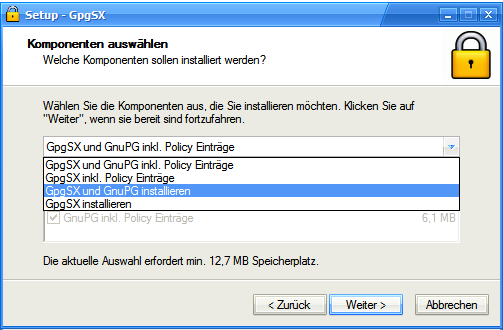
\includegraphics[scale=0.55]{../screenshots/gpgsx1.png}
\caption{GpgSX Installation}
\label{abb:gpgsx}
\end{center}
\end{figure}

 Nach dem Download ist das Setup-Programm zu starten und den Anweisungen zu folgen. Die Komponenten GnuPG und GpgSX sind zu installieren.

 \end{description}
\subsection{Installation der Enigmail-Erweiterung}
Enigmail \footnote{ \href{http://enigmail.mozdev.org/}{http://enigmail.mozdev.org}} ist eine Erweiterung f�r Mozilla Thunderbird, welche eine Schnittstelle zu GnuPG bereitstellt und den Umgang mit Verschl�sselung im t�glichen E-Mail Chaos vereinfacht. Am einfachsten installiert man Enigmail mit dem Add-on Manager von Thunderbird. Den Manager findet man unter \textit{Extras - Add-ons}. Im Suchfeld gibt man \textit{Enigmail} ein. Ein Klick auf den Button \textit{Installieren} holt das Add-on.

\begin{figure}[htb]
\begin{center}
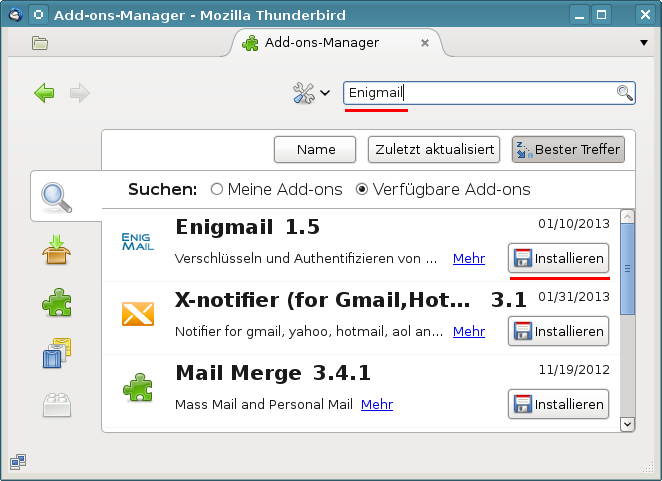
\includegraphics[scale=0.75]{../screenshots/enigmail_inst.png}
\caption{Installation von EnigMail}
\label{abb:enigmailinst}
\end{center}
\end{figure}

Nach Installation von Enigmail muss Thunderbird neu gestartet werden! Nach dem Neustart kann man den Konfigurations-Assistenten unter \textit{OpenPGP - OpenPGP-Assistent} aufrufen. Dabei werden folgende Schritte durchlaufen:

\begin{enumerate}
 \item Abfrage, ob gesendete E-Mails standardm��ig signiert und verschl�sselt werden sollen. Um unbedarfte Anwender nicht zu verwirren, kann man diese Funktion deaktivieren.
\item Abfrage, ob gesendete E-Mails standardm��ig verschl�sselt werden sollen. Da man meist nur OpenPGP-Schl�ssel von wenigen Empf�ngern hat, kann man diese Option zun�chst deaktivieren. Sp�ter, wenn sich die Verschl�sselung im Bekanntenkreis durchgesetzt hat, ist eine Aktivierung vielleicht sinnvoll.
\item Optimierung der Einstellungen f�r GnuPG. Die Vorgaben sind sinnvoll und sollten �bernommen werden.
\item Generieren der Schl�sselpaare f�r alle vorhandenen Konten. Die Passphrase f�r den Zugriff auf den privaten Key sollte man sich vorher gut �berlegen und merken! Es hei�t \textit{Passphrase} und nicht \textit{Passwort}. Die Passphrase darf ruhig etwas l�nger sein und auch Leer- bzw. Sonderzeichen enthalten.\\

Die Vorschl�ge des Assitenten sind erst einmal sinnvoll. Individuelle Anpassungen (z.B. 4096 Bit Schl�ssell�nge usw.) kann man nur beim Erstellen eines neuen Schl�ssels in der Schl�sselverwaltung w�hlen.\\

Kryptografischen Funktionen k�nnen nicht unbegrenzt den Fortschritten der Kryptoanalys widerstehen. Es ist sinnvoll, die Nutzungszeit des Schl�ssels mit einem Haltbarkeitsdatum zu versehen. Eine Nutzung l�nger als \textbf{5 Jahre} sollte man nur in begr�ndeten Ausnahmen in Erw�gung ziehen. Bei der Schl�sselerstellung sollte ein Verfallsdatum angegeben werden.\\

 Mit jedem Schl�sselpaar kann auch ein Zertifikat f�r den R�ckruf erstellt und sicher gespeichert werden. Mit diesem Zertifikat kann man einen Schl�ssel f�r ung�ltig erkl�ren, wenn der private Key kompromittiert wurde oder die Passphrase in Vergessenheit ger�t.\\
Dieser 4. Schritt kann �bersprungen werden, wenn man bereits g�ltige OpenPGP Schl�ssel hat.
\item FERTIG
\end{enumerate}

Sollte Enigmail das Programm \textit{gpg} nicht finden, weil man lieber die Version 2 \textit{gpg2} von GnuPG nutzen m�chte oder weil man es unter WINDOWS in einem selten verwendeten Verzeichnis liegt, w�hlt man den Men�punkt \textit{OpenPGP / Einstellungen} und gibt in der Dialogbox den Pfad zum GPG-Programm ein.

\subsection{Schl�sselverwaltung}
Die Schl�sselverwaltung findet man in Thunderbird unter dem Men�punkt \textit{OpenPGP - Sch�ssel verwalten}. Ist die Liste noch leer, w�hlt man zuerst den Men�punkt \textit{Erzeugen - Neues Schl�sselpaar}. Diesen Schritt �bernimmt jedoch auch der Assistent zur Einrichtung von Enigmail.

\begin{figure}[htb]
\begin{center}
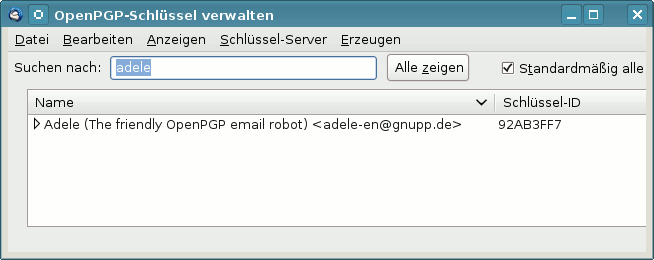
\includegraphics[scale=0.75]{../screenshots/enigmail_schl.png}
\caption{Schl�sselverwaltung von EnigMail}
\label{abb:enigmail_schl}
\end{center}
\end{figure}

\subsubsection*{Exportieren des eigenen �ffentlichen Schl�ssels}
Um verschl�sselt zu kommunizieren, muss den Kommunikationspartnern der eigene �ffentliche Schl�ssel zur Verf�gung gestellt werden. Der einfachste Weg nutzt die Schl�sselserver im Internet. In der Schl�sselverwaltung findet man den Men�punkt \textit{Schl�ssel-Server / Schl�ssel hochladen}. Der �ffentliche Schl�ssel wird auf den Schl�sselserver exportiert und steht dort allen Partnern zur Verf�gung. Die verschiedenen Server synchronisieren ihren Datenbestand.\\

Alternativ k�nnte man den �ffentlichen Schl�ssel als E-Mail Attachment versenden oder als Datei auf einem Webserver ablegen. Den Men�punkt f�r den Export in eine Datei findet man unter \textit{Datei - Schl�ssel exportieren} in der Schl�sselverwaltung. Um den Schl�ssel als Attachment an eine Mail anzuh�ngen, aktivieren Sie die Option \textit{OpenPGP - Meinen �ffentlichen Schl�ssel anh�ngen} beim Schreiben einer Mail wie im Bild \ref{abb:enigmailaddkey} zu sehen.

\begin{figure}[htb]
\begin{center}
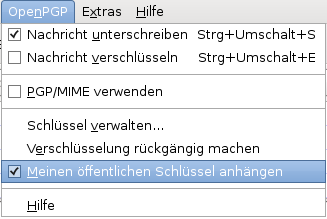
\includegraphics[scale=0.75]{../screenshots/enigmail_add_key.png}
\caption{OpenPGP-Schl�ssel versenden}
\label{abb:enigmailaddkey}
\end{center}
\end{figure}

\subsubsection*{Import der Schl�ssel der Partner}
Um an einen Kommunikationspartner verschl�sselte E-Mails zu senden oder die Signatur erhaltener Nachrichten zu pr�fen, ben�tigt man den �ffentlichen Schl�ssel des Partners.

\begin{itemize}
 \item Am einfachsten l��t sich dieser importieren, wenn man eine signierte E-Mail erhalten hat. Ein Klick auf den blauen Stift rechts oben im Header der E-Mail reicht aus, um den �ffentlichen Schl�ssel von einem Schl�sselserver zu importieren.
\item Zum Importieren des Schl�ssel eines Partners aus einer Datei, die man als Attachement oder per Download erhalten hat, w�hlt man den Men�punkt \textit{Datei / Importieren} in der Schl�selverwaltung.
\item Wenn der Schl�ssel als Text angeboten wird, sieht es etwa so aus:
\begin{verbatim}
 -----BEGIN PGP PUBLIC KEY BLOCK-----
 Version: SKS 1.1.1
 
 mQENBEt5GIIBCACOnOeTtfBIUbdcOmw5DlLuxkQB4uQ/8HbSUaH96s1z
 HqFA/31GB70podyEKqc41T2TDdWWITfdy1dpxeGwopBK/wljPAuNAgJQ
 ....
 fU7xEW/RQT76n0RfTXnbj2m/DRPmoivcXW5G/zJM6QUjl++vO7OB+3xb
 SnDCMQtaWHM57eLcmnsMAK3qHOYlVrNUTSvEgatjUqLU
 =fP9T
 -----END PGP PUBLIC KEY BLOCK-----
\end{verbatim} 
Man kann die Zeilen von BEGIN ...bis... END mit der Maus markieren und in die Zwischen�ablage kopieren. In der Schl�ssel�verwaltung von Enigmail importiert man den Schl�ssel wie im Bild \ref{abb:enigmailimp} dargestellt mit \textit{Bearbeiten - Aus Zwischenablage importieren}.

\begin{figure}[htb]
\begin{center}
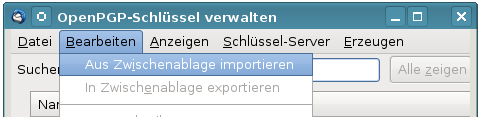
\includegraphics[scale=0.75]{../screenshots/enigmail-clip.png}
\caption{OpenPGP-Schl�ssel aus Zwischenablage importieren}
\label{abb:enigmailimp}
\end{center}
\end{figure}

\item Auch ohne eine signierte E-Mail erhalten zu haben, kann man die Schl�sselserver nach dem zu einer E-Mail Adresse geh�renden Schl�ssel durchsuchen. Die Funktion findet man unter dem Men�punkt \textit{Schl�ssel-Server / Schl�ssel suchen}. Man gibt in der sich �ffnenden Dialogbox die E-Mail-Adresse des Empf�ngers ein und best�tigt mit Ok.\\

Wurden zur Suchanfrage passende Schl�ssel gefunden, werden diese in einer Liste angezeigt. W�hlen Sie aus dieser Liste den zu importierenden Schl�ssel und best�tigen Sie mit OK. Wenn mehrere passende Schl�ssel f�r eine E-Mail Adresse gefunden wurden, ist in der Regel der neueste Schl�ssel die richtige Wahl.

\begin{figure}[htb]
\begin{center}
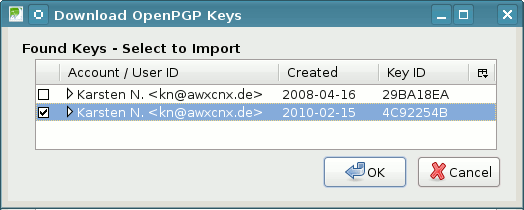
\includegraphics[scale=0.75]{../screenshots/enigmail_suche2.png}
\caption{Mehrere OpenPGP-Schl�ssel gefunden}
\label{abb:enigmailsuche}
\end{center}
\end{figure}

\end{itemize}


\subsection{Signieren und Verschl�sseln erstellter E-Mails}
Wurde in den Kontoeinstellungen in der Sektion \textit{OpenPGP} die Option  \textit{Nachrichten standardm��ig verschl�sseln} aktiviert, sind beim Schreiben einer E-Mail keine weiteren Hinweise zu beachten. Anderenfalls ist f�r jede E-Mail explizit festzulegen, dass sie verschl�sselt werden soll.\\

Das Fenster f�r das Erstellen einer neuen E-Mail (Bild \ref{abb:thunder_email_neu}) zeigt nach der Installation des Enigmail-PlugIns einen neuen Button \textit{OpenPGP}. Klickt man auf diesen Button, �ffnet sich der im Bild \ref{abb:thunder_email_neu} gezeigte Dialog, der es erm�glicht, die Krypto-Eigenschaften f�r diese E-Mail festzulegen.\\

Sollte die E-Mail Anh�nge enthalten, ist die Option \textit{PGP / MIME} zu aktivieren, um die Attachements standardkonform zu verschl�sselt.\\

\textbf{Achtung:} Die Betreffzeile wird nicht (!) mit verschl�sselt. Sicher wird man die Kontonummer nicht in der Betreffzeile schreiben, aber auch ein ausf�hrlicher Betreff erm�glicht zusammen mit der/den Adressen der Empf�nger einige Aussagen �ber die Kommunikation.\\

Wenn man als Betreff beispielsweise schreibt:
\begin{quote}
 \textit{Treffen der Aktivisten-Gruppe ... am 13.01.09}
\end{quote} 

und diese Mail per CC an alle Mitglieder der Gruppe versendet, sind 90\% der relevanten Informationen bekannt und man kann sich die Verschl�sselung der Mail sparen.\\

Soll jede versendete E-Mail verschl�sselt werden, wenn der Schl�ssel des Empf�ngers vor�handen ist, kann die entsprechende Option in den Konto Einstellungen unter \textit{OpenPGP -> Sicherheit} aktiviert werden. Alternativ ist es auch m�glich, lediglich f�r bestimmte Empf�nger festzulegen, dass alle E-Mails signiert oder verschl�sselt werden sollen. Diese Regeln kann man unter \textit{OpenPGP -> Empf�ngerregeln} definieren.

\begin{figure}[htb]
\begin{center}
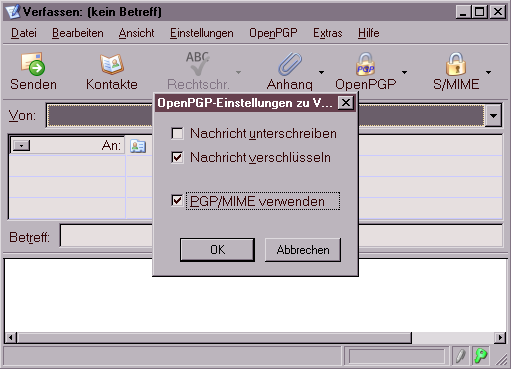
\includegraphics[scale=0.55]{../screenshots/gpg_senden.png}
\caption{Signieren und Verschl�sseln einer E-Mail}
\label{abb:thunder_email_neu}
\end{center}
\end{figure}

\subsection{Adele - der freundliche OpenPGP E-Mail-Roboter}
Adele ist der freundliche OpenPGP E-Mail-Roboter der G-N-U GmbH. Man kann mit dem Robot seine ersten verschl�sselten Mails austauschen und ein wenig �ben ohne Freunde mit Anf�nger�probleme zu bel�stigen.

\begin{description}
 \item[1: Den eigenen Schl�ssel an Adele senden:] Als erstes schickt man den eigenen �ffentlichen Schl�ssel per E-Mail an \textit{adele@gnupp.de}. Den Schl�ssel h�ngt man als Anhang an die Mail an, indem man die Option \textit{OpenPGP - Meinen �ffentlichen Schl�ssel anh�ngen} vor dem Versenden der Mail aktiviert (Bild \ref{abb:enigmailaddkey})

 \item[2. Verschl�sselte Antwort von Adele:] Als Antwort erh�lt man nach einigen Minuten eine verschl�sselte E-Mail von Adele. Die E-Mail wird nach Abfrage der Passphrase entschl�sselt und enth�lt den Schl�ssel von Adele:

\begin{verbatim}
 Hallo,
 
 hier ist die verschl�sselte Antwort auf Ihre E-Mail.
 
 Ihr �ffentlicher Schl�ssel wurde von mir empfangen.
 
 Anbei der �ffentliche Schl�ssel von adele@gnupp.de,
 dem freundlichen E-Mail-Roboter.
 
 Viele Gr��e,
 adele@gnupp.de
 
 -----BEGIN PGP PUBLIC KEY BLOCK-----
 Version: GnuPG v1.4.9 (GNU/Linux)
 
 mQGiBDyFlIkRBACfVHJxv47r6rux7TwT4jHM7z/2VfyCrmcRegQEsbdLfqu3mEmK
 RouuaDQukNINWk2V2ErOWzFnJqdzpapeuPJiOWp0uIEvU3FRPhYlytw9dFfwAHv4
 MJ7639tAx9PfXBmZOd1PAoE451+VLhIGlLQiFGFppJ57SZ1EQ71/+/nkSwCg8Mge
 ....
 EQIABgUCPIWUlQASCRDlczRpkqs/9wdlR1BHAAEBv20AoJJGeeZjMCSbXtmNSwfW
 QsLOd0+4AKCdXwt552yi9dBfXPo8pB1KDnhtbQ==
 =ERT8
 -----END PGP PUBLIC KEY BLOCK-----
\end{verbatim} 

\item[3. Schl�ssel von Adele importieren:] Man kann die Zeilen von \texttt{BEGIN PGP PUBLIC KEY BLOCK} bis einschlie�lich \texttt{END PGP PUBLIC KEY BLOCK} mit der Maus markieren, in die Zwischenablage kopieren und in der Schl�sselverwaltung �ber \textit{Bearbeiten - Aus Zwischenablage importieren} einf�gen.\\

 Alternativ holt man sich Adeles Schl�ssel mit der ID 0x92AB3FF7 von einem Keyserver.

\item[4. Adele verschl�sselte E-Mails schreiben] Jetzt kann man Adele verschl�sselte E-Mails schicken. Als Antwort erh�lt man umgehend eine gleichfalls verschl�sselte E-Mail mit dem gesendeten Text als Zitat.
\begin{verbatim}
 Hallo,
 
 hier ist die verschl�sselte Antwort auf Ihre E-Mail.
 
 Ich schicke Ihnen Ihre Botschaft im Wortlaut zur�ck, damit Sie
 sehen, dass ich sie erfolgreich entschl�sseln konnte.
 
 > Hello Adele,
 >
 > hope you are feeling well.
\end{verbatim} 

 \end{description}

\subsection{Verschl�sselung in Webformularen}
Auch bei der Nutzung eines Webmail Accounts oder Webforms f�r die Versendung anonymer E-Mails muss man auf Verschl�sselung nicht verzichten.\\

Einige grafische Tools f�r die Schl�sselverwaltung wie z.B. GPA (\textit{GNU Privacy Assistent}) \footnote{ \href{http://www.gnupg.org/related\_software/gpa/index.de.html}{http://www.gnupg.org/related\_software/gpa/index.de.html}} oder KGPG enthalten einen Editor. Man kann den Text in diesem Editor schreiben, mit einem Klick auf den entsprechenden Button signieren oder verschl�sseln und das Ergebnis �ber die Zwischenablage in die Textbox der Website einf�gen. Entschl�sseln funktioniert umgekehrter.\\

Enth�lt das bevorzugte Tool f�r die Schl�sselverwaltung keinen Texteditor, kann man folgende Alternativen nutzen, die auch f�r unterwegs (auf dem USB-Stick) geeignet sind:
\begin{enumerate}
 \item Das kleine Tool \textbf{gpg4usb} \footnote{ \href{http://gpg4usb.cpunk.de}{http://gpg4usb.cpunk.de}} bietet einen Editor mit den Buttons f�r das Ver- und Entschl�sseln des Textes, Dateiverschl�sselung sowie eine kleine Schl�sselverwaltung (Signieren und Pr�fen der Signatur steht noch auf der ToDo Liste). Das ZIP-Archiv enth�lt Versionen f�r Windows und Linux. Es kann einfach auf dem USB-Stick genutzt werden.
\item Die Applikation \textbf{Portable PGP} \footnote{ \href{http://ppgp.sourceforge.net/}{http://ppgp.sourceforge.net}} ist eine Java-Anwendung (plattformunabh�ngig), die ebenfalls Texte und Dateien ver- und entschl�sseln kann. Eine einfach Schl�sselverwaltung ist ebenfalls  enthalten. Zus�tzlich zu Portable PGP ben�tigt man eine Java Laufzeitumgebung. Eine portable Version der Sun-JRE gibt es bei portableapps.com.
\end{enumerate}

\subsection{GnuPG SmartCard nutzen}
Die Sicherheit asymmetrischer Verschl�sselung h�ngt in hohem Ma�e von der sicheren Aufbewahrung des privaten Keys ab. Nutzt man GnuPG auf mehreren Rechnen, insbesondere wenn andere Nutzer Administrator- bzw. Root-Privilegien auf diesen Rechnern haben, k�nnte der private Key in falsche H�nde gelangen.\\

B�swillige Buben k�nnten mit einem Trojaner versuchen, den privaten Key zu kopieren und das Passwort mit Tools wie \textit{Elcomsoft Distributed Password Recovery} \footnote{ \href{http://www.elcomsoft.de/programme/edpr.html}{http://www.elcomsoft.de/programme/edpr.html}} ermitteln. Die unbedachte Entsorgung einer Festplatte oder eines Computers ist ein weiteres Risiko, wenn der private Key nicht zuverl�ssig gel�scht wurde.\\

\textbf{SmartCards:} erm�glichen eine sichere Nutzung von GnuPG unter diesen Bedingungen. Der private Key ist ausschlie�lich auf der SmartCard gespeichert, er verl��t diese sichere Umgebung nicht. S�mtliche kryptografischen Operationen werden auf der Card ausgef�hrt. CardReader (USB) und GnuPG-SmartCards gibt es bei kernelconcepts.de \footnote{\href{http://www.kernelconcepts.de/shop/products/security.shtml?hardware}{http://www.kernelconcepts.de/shop/products/security.shtml?hardwaree}}.\\

\textbf{CryptoStick:} Da das Handling mit CardReader und SmartCard unter Umst�nden etwas umst�ndlich sein kann, wurde ein USB-Stick entwickelt, der CardReader plus eine SmartCard in einem kleinen Geh�use enth�lt und voll kompatibel mit der Version 2.0 der OpenPGP SmartCard ist. Weitere Informationen gibt es auf der Webseite des Projektes \footnote{ \href{http://www.crypto-stick.com}{http://www.crypto-stick.com}}.

\begin{figure}[htb]
\begin{center}
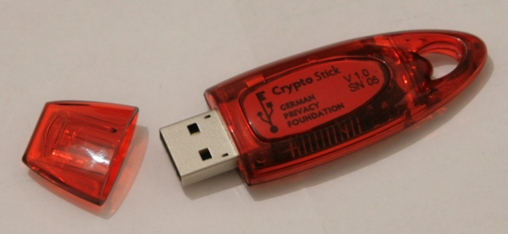
\includegraphics[scale=0.6]{../screenshots/cryptostick2.jpeg}
\caption{CryptoStick}
\label{abb:cryptostick}
\end{center}
\end{figure}

\subsubsection*{Hardware-Treiber installieren}
Vor der Nutzung der SmartCard ist der Hardware-Treiber f�r den CardReader zu installieren.
\begin{itemize}
   \item WINDOWS: Die Lieferung des CardReaders von kernelconcepts.de enth�lt eine CD mit den n�tigen Treiber f�r WINDOWS. Das zum Ger�t passende ZIP-Archiv ist zu entpacken und \textit{setup.exe} als Administrator zu starten.\\

   F�r den CryptoStick gibt es den PC Twin USB PC/SC Treiber \footnote{ \href{http://support.gemalto.com/?id=46}{http://support.gemalto.com/?id=46}}.

\item Linux: Da Linux out-of-the-box viel mehr Hardware unterst�tzt als Windows, sind die n�tigen Treiber in den Repositories enthalten. Unter Debian/Ubuntu installiert man alles N�tige f�r die Nutzung der SmartCard mit folgendem Kommando: 
\begin{verbatim}
  # aptitude install pcscd libpcsclite1 libccid
\end{verbatim}

Die Pakete \textit{openct} und \textit{opensc} sollten entfernt werden, da diese zu Beeintr�chtigungen f�hren k�nnen. 
\end{itemize}
\begin{verbatim}
  # aptitude purge openct opensc
\end{verbatim}


Au�erdem ben�tigen die aktuelle OpenPGP-SmartCard und der Crypto-Stick GnuPG mindestens in der Version 1.4.9+ oder die 2.0.12+. Unter WINDOWS funktioniert erst die Version 1.4.10. Aktualisieren sie ihre GnuPG Version, wenn n�tig.\\

Wer ``gpg2'' nutzen m�chte, sollte beachten, dass der ``gpg-agent'' unbedingt n�tig ist. In der Datei \textit{\$HOME/.gnupg/gpg.conf} ist am Ende einfach ein \texttt{use-agent} einzuf�gen. Dann meldet man sich vom Desktop ab und wieder an.\\

Nachdem die Software installiert wurde, sollte man pr�fen, ob alles funktioniert. SmartCard anschlie�en und auf der Konsole bzw. DOS-Box eingeben: 
\begin{verbatim}
  > gpg --card-status
  Application ID ...: D27600xxxxxxxxxxxxxxx
  Version ..........: 2.0
  Manufacturer .....: unknown
  .... 
\end{verbatim}

\subsubsection*{SmartCards und CryptoStick mit Enigmail nutzen}
Enigmail ist seit der Version 1.0.1 voll kompatibel mit der SmartCard und dem CryptoSick. Das Add-on bietet eine grafische Oberfl�che, um die SmartCard zu verwalten. Diese Funktionen �ffnet man �ber den Men�punkt \textit{OpenPGP - Smartcard verwalten}.

\begin{figure}[htb]
\begin{center}
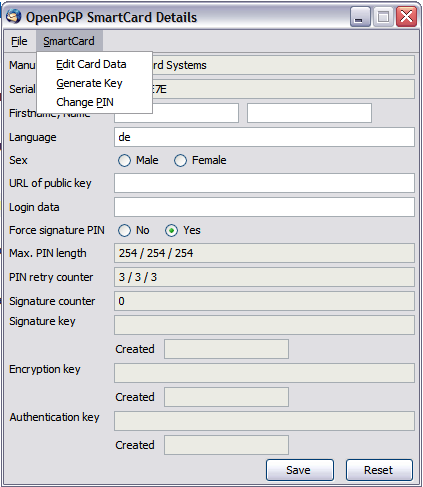
\includegraphics[scale=0.55]{../screenshots/smartcard1.png}
\caption{SmartCard verwalten}
\label{abb:smartcard1}
\end{center}
\end{figure}

\begin{enumerate}
 \item Als Erstes kann man die Card personalisieren und den Namen usw. editieren, eine URL f�r den Public Key angeben... (\textit{Edit Card Data}).

\item Im zweiten Schritt sollte der PIN und der Admin-PIN ge�ndert werden. Der PIN ist eine 6-stellige Zahlenkombination (Default: 123456), welche den User-Zugriff auf die Card sichert. Der Admin-PIN ist eine 8-stellige Zahlenkombination (Default: 12345678) f�r die Verwaltungsoperationen.\\

Wurde der PIN 3x falsch eingegeben, wird die Card gesperrt und kann mit dem Admin-PIN wieder entsperrt werden (\textit{Unblock PIN}). Wird der Admin-PIN 3x falsch eingegeben, ist die SmartCard zerst�rt!.\\

Die Festlegung auf 6- bzw. 8-stellige Zahlenkombinationen legt es nahe, ein Datum aus dem pers�nlichen Leben als PINs zu nutzen. Das reduziert die Vergesslichkeit. Es sollte jedoch kein einfach zu erratenes Datum wie der Geburtstag des T�chterchens sein.

\begin{figure}[htb]
\begin{center}
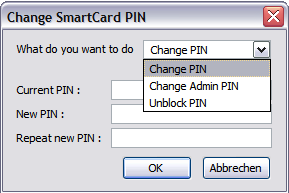
\includegraphics[scale=0.55]{../screenshots/smartcard3.png}
\caption{SmartCard-PINs �ndern}
\label{abb:smartcard3}
\end{center}
\end{figure}

\item Als letzten Schritt vor der Nutzung der SmartCard im t�glichen Krypto-Chaos sind die Keys auf der SmartCard zu generieren. Der entsprechende Dialog bietet die Auswahl eines Mail-Account an, f�r den die SmartCard genutzt werden soll. F�r diesen Account darf kein(!) OpenPGP-Key vorhanden sein. Anderenfalls bricht der Vorgang mit einer wenig verst�ndlichen Fehlermeldung ab.\\

Es sollte unbedingt bei der Erzeugung des Schl�ssels ein Backup der Card-Keys angelegt und mit einem Passwort gesichert werden. Sp�ter ist kein Zugriff auf diese Schl�ssel mehr m�glich. Bei Besch�digung der SmartCard kann der gesicherte Card-Key in eine neue SmartCard importiert werden. Das Backup wird im GnuPG-Verzeichnis abgelegt und ist auf einem sicheren Datentr�ger zu speichern!\\

Wurden die Schl�ssel erfolgreich generiert, findet man in der \textit{Schl�sselverwaltung} ein neues Paar. Der Public Key dieses Schl�sselpaares kann wie �blich exportiert und den Partnern zur Verf�gung gestellt werden. Der Private Key dieses Paares definiert lediglich, dass die kryptografischen Operationen auf einer SmartCard auszuf�hren sind. Er ist ohne die passende Card unbrauchbar.
\end{enumerate}

\subsubsection*{Funktionen f�r Genie�er}
Die Nutzung von gpg auf der Kommandozeile bietet etwas mehr M�glichkeiten, als bisher im Enigmail-GUI implementiert sind. Nat�rlich stehen auch die mit dem GUI durchf�hrbaren Funktionen auf der Kommandozeile zur Verf�gung.\\

Einen �berblick �ber alle SmartCard-Funktionen gibt die Hilfe. Als erstes muss man den Admin Mode aktivieren, dann hat man vollen Zugriff auf alle Funktionen:
\begin{verbatim}
   > gpg --card-edit
   Befehl> admin
   Befehl> help
\end{verbatim} 

Neue Schl�ssel generiert man auf der SmartCard mit:
\begin{verbatim}
   > gpg --card-edit
   Befehl> admin
   Befehl> generate
\end{verbatim} 

Hat man mehrmals den PIN falsch eingegeben kann man ein neuen (alten) PIN (r�ck-)setzen, wenn man den Admin-PIN kennt:
\begin{verbatim}
   > gpg --card-edit
   Befehl> admin
   Befehl> passwd
\end{verbatim} 

M�glicherweise hat man bereits eine OpenPGP Schl�ssel mit vielen Signaturen. Den m�chte man nicht wegwerfen und im Web of Trust noch einmal von vorn beginnen. Als Ausweg bietet es sich an, einen vorhandenen, starken Schl�ssel mit der SmartCard zus�tzlich zu sch�tzen. Der Zugriff auf den geheimen Schl�ssel ist dann nur mit der SmartCard m�glich. Es ist dem vorhanden Schl�ssel mit der ID key-id ein Subkey der SmartCard hinzuzuf�gen. Das geht nur auf der Kommandozeile:
\begin{verbatim}
   > gpg --edit-key key-id
   command> addcardkey
\end{verbatim}

Dabei wird ein evtl. auf der SmartCard vorhandener Key zert�rt!

\subsection{SSL-Verschl�sselung f�r Keyserver aktivieren}
Seit Anfang Oktober 2012 bietet der Keyserverpool sks-keyservers.net einen Sub-Pool mit SSL-Verschl�sselung f�r das Abrufen und Senden von OpenPGP-Schl�sseln \footnote{ \href{http://permalink.gmane.org/gmane.comp.encryption.pgp.sks/3559}{http://permalink.gmane.org/gmane.comp.encryption.pgp.sks/3559}}. Die SSL-Verschl�sselung verhindert, dass ein Lauscher beobachtet, welche OpenPGP-Schl�ssel man sucht und herunter l�dt.\\

Um diesen sicheren Sub-Pool zu nutzen, sind folgende Schritte n�tig:
\begin{enumerate}
 \item Man ben�tigt eine Version von GnuPG, die das \textit{hkps://} Protokoll unterst�tzt. Man kann \textit{gnupg2} nutzen oder das Paket \textit{gnupg-curl} installieren. F�r Windows bietet \textit{gpg4win} ein Paket mit \textit{gnupg2}, unter Linux installiert man eines der genannten Pakete mit dem bevorzugten Paketmanager.
 \item Das CA-Root Zertifikat des Keyserverpool \textit{sks-keyservers.netCA.pem}\footnote{ \href{https://sks-keyservers.net/sks-keyservers.netCA.pem}{https://sks-keyservers.net/sks-keyservers.netCA.pem}} ist herunter zu laden und auf dem eigenen Rechner zu speichern.
 \item In der Konfiguration von Enigmail sind die \textit{Experten Optionen} zu aktivieren und folgende Werte einzutragen:
\begin{enumerate}
 \item Bei der Nutzung von \textit{gnupg2} ist der Pfad zu diesem Programm auszuw�hlen.
 \item Auf dem Reiter \textit{Schl�ssel-Server} ist der HKPS-Pool als einziger Schl�ssel-Server einzutragen:
   \begin{verbatim}
hkps://hkps.pool.sks-keyservers.net
   \end{verbatim} 
 \item Auf dem Reiter \textit{Erweitert} sind als \textit{Zus�tzliche Parameter f�r GnuPG} die n�tigen Keyserver-Optionen einzutrage:
   \begin{verbatim}
--keyserver-options ca-cert-file=<Path to>/sks-keyservers.netCA.pem
   \end{verbatim} 
\end{enumerate}

\end{enumerate}


\subsection{Web des Vertrauens}
Im Prinzip kann jeder Anwender einen Schl�ssel mit beliebigen E-Mail Adressen generieren. Um Vertrauen zu schaffen, gibt es das \textbf{Web of Trust}.\\

Hat Beatrice die Echtheit des Schl�ssels von Anton �berpr�ft, kann sie diesen mit ihrem geheimen Schl�ssel signieren und auf die Schl�sselserver re-exportieren. Conrad, der den Schl�ssel von Beatrice bereits �berpr�ft hat, kann damit aufgrund der Signatur auch dem Schl�ssel von Anton vertrauen. Es bildet sich ein weltweites Netz von Vertrauensbeziehungen. Die Grafik Bild \ref{abb:weboftrust} zeigt eine m�gliche Variante f�r den Key von Anton (A).\\

\begin{figure}[htb]
\begin{center}
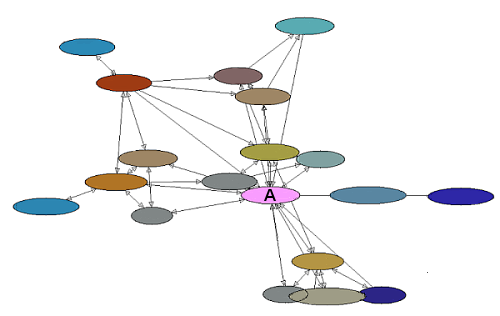
\includegraphics[scale=0.55]{../grafiken/web_of_trust.png}
\caption{Beispiel f�r ein Web of Trust}
\label{abb:weboftrust}
\end{center}
\end{figure}

\subsubsection*{OpenPGP-Schl�ssel signieren}

Die Echtheit eines Schl�ssels kann anhand des Fingerabdrucks gepr�ft werden. Zu jedem Schl�ssel existiert ein eindeutiger Fingerabdruck. Dieser l�sst sich in den Eigenschaften des Schl�ssels anzeigen. In der Schl�sselverwaltung ist der zu pr�fende Schl�ssel auszuw�hlen und �ber den Men�punkt \textit{Anzeigen - Eigenschaften} den im Bild \ref{abb:enigmail_schl_eigensch} dargestellten Dialog zu �ffnen.\\

Der angezeigte Fingerabdruck des Schl�ssels kann mit dem Wert verglichen werden, den man vom Eigent�mer des Schl�ssels erhalten hat. Sind beide identisch, kann das Vertrauen des �ffentlichen Schl�ssels auf ein hohes Niveau gesetzt werden. Den Dialog findet man in der Schl�sselverwaltung unter \textit{Bearbeiten - Vertrauensw�rdigkeit}.\\

\begin{figure}[htb]
\begin{center}
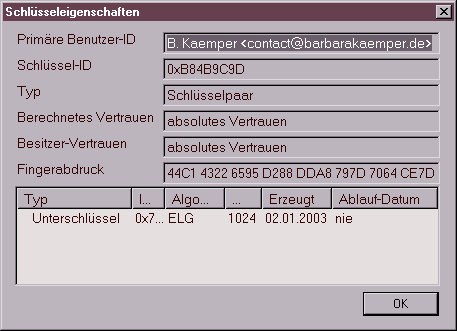
\includegraphics[scale=0.5]{../screenshots/schluessel_eigensch.png}
\caption{Schl�ssel-Eigenschaften}
\label{abb:enigmail_schl_eigensch}
\end{center}
\end{figure}

Hat man sich von der Echtheit des Schl�ssels �berzeugt, kann man ihn in Absprache mit dem Schl�sseleigent�mer auch signieren und den signierten Schl�ssel auf einen Keyserver exportieren. Wenn viele Nutzer die Ergbnisse ihrer �berpr�fung online verf�gbar machen, entsteht das Web-of-Trust und es wird schwer, gef�lschte Schl�ssel in Umlauf zu bringen.

\subsubsection*{Certification Authorities}
Diese Infrastruktur kann auch von vertrauensw�rdigen Institutionen (Certification Authorities, CAs) genutzt werden. Die Nutzer wenden sich an die CA und lassen gegen Vorlage von Ausweisdokumenten den eigenen OpenPGP-Key signieren. Alle Partner ben�tigen lediglich den �ffentlichen Schl�ssel der CA, um die Echtheit der Schl�ssel zu �berpr�fen.\\

Beispiele f�r Certification Authorities sind:
\begin{itemize}
\item CAcert.org signiert auch OpenPGP-Schl�ssel
\item Krypto-Kampagne der Zeitschrift c't
\item PCA des Deutschen Forschungsnetzes (DFN-PCA)
\end{itemize}

\subsubsection*{Keysigning-Party}
Wenn sich mehrere OpenPGP-Nutzer treffen um sich gegenseitig die Echtheit ihrer Schl�ssel zu best�tigen, nennt man es eine \textit{Keysigning-Party}. Dabei kommt es nicht darauf an, dass die Beteiligten sich pers�nlich kennen. Die Echtheit des Schl�ssels k�nnen auch Unbekannte gegen Vorlage von Ausweisdokumenten und Fingerprint des Key best�tigen.\\

Eine Keysigning-Party l�uft �blicherweise folgenderma�en ab:
\begin{enumerate}
   \item Der Organisator l�dt zu einer Party ein und bittet um Anmeldungen.
\item Wer an der Party teilnehmen m�chte, sendet seinen public OpenPGP-Key zusammen mit Namen und dem Fingerprint an den Organisator.
\item In Vorbereitung der Party erstellt der Organisator einen Keyring f�r alle Beteiligte und eine Liste mit Namen, Key-IDs und Fingerprints von allen Teilnehmern.
\item Der Keyring und die Liste werden an alle Teilnehmer verteilt. Die Teilnehmer k�nnen auf der Party die Identit�t gegenseitig durch Vorlage von Ausweisdokumenten pr�fen.
\item Wieder zuhause k�nnen die Schl�ssel im Party-Keyring signiert und an die Inhaber per E-Mail versendet werden. In der Regel erfolgt dieser Schritt nicht beim Treffen.
\end{enumerate}

Wer h�ufiger an Keysigning-Partys teilnimmt, kann unter Linux das Tool \textit{caff} f�r den letzten Schritt nutzen. Das Tool ist im Paket \textit{signing-party} f�r nahezu alle Linux-Ditributionen verf�gbar und kann mit dem Paket-Manager der Wahl installiert werden.\\

Nach der Installation ist die Datei \$HOME/.caffrc als Textdatei anzulegen und die Werte f�r den eigenen Namen, E-Mail Adresse, OpenPGP-ID sowie die Parameter zur Versendung von E-Mails sind zu konfigurieren:

\begin{verbatim}
$CONFIG{'owner'} = 'Michi M�ller';
$CONFIG{'email'} = 'm@m.de';
$CONFIG{'keyid'} = [ qw{01234567890ABCDE} ];

$CONFIG{'mailer-send'} =  [ 'smtp', Server => 'mail.server', Auth => ['user','pass'] ];
\end{verbatim} 

Ein kleines Kommando im Terminal signiert alle Schl�ssel des Party-Keyring, verpackt sie in E-Mails, die mit dem
Key der Empf�nger verschl�sselt werden, und sendet die E-Mails an die Inhaber der OpenPGP-Keys:

\begin{verbatim}
 > caff --key-file party-keyring.asc
\end{verbatim} 

\subsection{Schl�ssel zur�ckrufen}
Soll ein Schl�sselpaar nicht mehr verwendet werden (beispielsweise weil der geheime Schl�ssel kompromittiert wurde
oder die Passphrase in Vergessenheit gefallen ist), kann der �ffentliche Schl�ssel f�r ung�ltig erkl�rt werden.\\

�ffnen Sie die Schl�sselverwaltung, w�hlen Sie den Schl�ssel, der f�r ung�ltig erkl�rt werden soll. Rufen Sie den Men�punkt \textit{Bearbeiten / zur�ckrufen} auf. Nach einer Sicherheitsfrage und Eingabe der Passphrase wird der Schl�ssel auf den Schl�sselservern im Internet f�r ung�ltig erkl�rt. Auch wenn der geheime Schl�ssel nicht mehr vorliegt oder die Passphrase in Vergessenheit geraten ist, kann der �ffentliche Schl�ssel f�r ung�ltig erkl�rt werden, indem das unter Punkt 4 erstellte R�ckrufzertifikat importiert wird.


\section{Eine Bemerkung zum Abschlu�}
\textit{``Mache ich mich verd�chtig, wenn ich meine E-Mails verschl�ssel?''}\\

Eine Frage, die h�ufig gestellt wird, wenn es um verschl�sselte E-Mails geht. Bisher gab es darauf folgende Antwort:\\

\textit{``Man sieht es einer E-Mail nicht an, ob sie verschl�sselt ist oder nicht. Wer bef�rchtet, dass jemand die Mail beschn�ffelt und feststellen k�nnte, dass sie verschl�sselt ist, hat einen Grund mehr, kryptografische Verfahren zu nutzen!''}\\

Aktuelle Ereignisse zeigen, dass diese Frage nicht mehr so einfach beantwortet werden kann. Dem promovierten Soziologen Andrej H. wurde vorgeworfen, Mitglied einer terroristischen Vereinigung nach �129a StGB zu sein. Der Haftbefehl gegen ihn wurde unter anderem mit \textbf{konspirativem Verhalten} begr�ndet, da er seine E-Mails verschl�sselte.\\

Am 21.Mai 2008 wurden in �stereich die Wohnungen von Aktivisten der Tierrechtsszene durchsucht und 10 Personen festgenommen. Der Haftbefehl wurde mit Verdunklungsgefahr begr�ndet, da die Betroffenen z.B. �ber verschl�sselte E-Mails kommunizierten.\\

Am 18.10.07 hat der Bundesgerichtshof (BGH) in seinem Urteil \href{http://juris.bundesgerichtshof.de/cgi-bin/rechtsprechung/document.py?Gericht=bgh&Art=pm&Datum=2007&Sort=3&anz=154&pos=0&nr=41487&linked=bes&Blank=1&file=dokument.pdf}{Az.: StB 34/07} den Haftbefehl gegen Andrej H. aufgehoben und eindeutig festgestellt, dass die Verschl�sselung von E-Mails als Tatverdacht NICHT ausreichend ist, entscheidend sei der Inhalt: \\

\textit{``Ohne eine Entschl�sselung der in den Nachrichten verwendeten Tarnbegriffe und ohne Kenntnis dessen, was bei den - teilweise observierten und auch abgeh�rten - Treffen zwischen dem Beschuldigten und L. besprochen wurde, wird hierdurch eine mitgliedschaftliche Einbindung des Beschuldigten in die 'militante gruppe' jedoch nicht hinreichend belegt.''}\\

Au�erdem geben die Richter des 3. Strafsenat des BGH zu bedenken, dass Andrej H. \textit{``ersichtlich um seine �berwachung durch die Ermittlungsbeh�rden wusste''}. Schon allein deshalb konnte er \textit{``ganz allgemein Anlass sehen''}, seine Aktivit�ten zu verheimlichen. Woher Andrej H. von der �berwachung wusste, steht bei \href{http://annalist.noblogs.org/}{http://annalist.noblogs.org}.\\

Trotz dieses Urteils des BGH bleibt f�r uns ein bitterer Nachgeschmack �ber die Arbeit unser Ermittler und einiger Richter. Zumindest die Ermittlungsrichter sind der Argumentation der Staatsanwaltschaft gefolgt und haben dem Haftbefehl erst einmal zugestimmt.
\end{document}